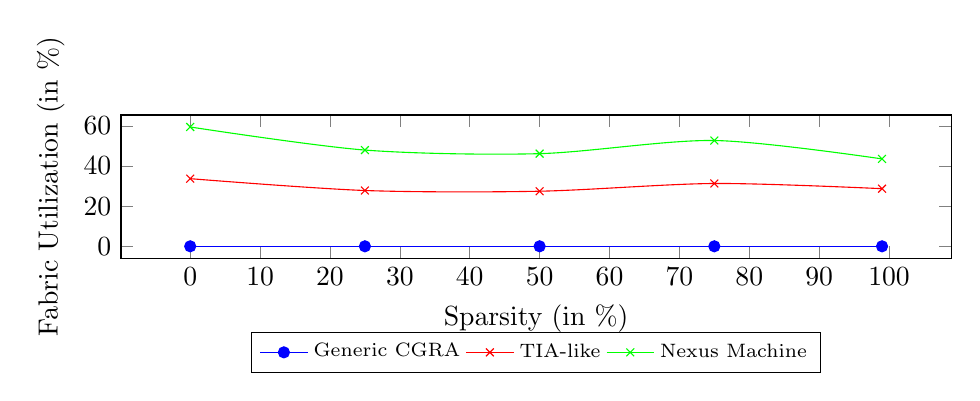
\begin{tikzpicture}
\begin{axis}[
    width=\columnwidth, height=3.4cm,
    xlabel=Sparsity (in \%),
    ylabel=Fabric Utilization (in \%),
    %xlabels at=edge bottom,
    %xticklabels at=edge bottom,
    %typeset ticklabels with strut,
    legend columns=4,
    legend columns=4,
    legend style={at={(0.5,-0.8,1.15)},
    anchor=south, font=\scriptsize},
    ]
    
\addplot[smooth,mark=*,blue] plot coordinates {
        (99,0)
        (75,0)
        (50,0)
        (25,0)
        (0,0)
};
\addlegendentry{Generic CGRA}

\addplot[smooth,color=red,mark=x]
    plot coordinates {
        (99,28.70813397)
        (75,31.29106188)
        (50,27.4408218)
        (25,27.79652031)
        (0,33.69159903)
    };
\addlegendentry{TIA-like}

\addplot[smooth,color=green,mark=x]
    plot coordinates {
        (99,43.53772348)
        (75,52.70200721)
        (50,46.15384615)
        (25,47.94363149)
        (0,59.43697398)
    };
\addlegendentry{Nexus Machine}

\end{axis}
\end{tikzpicture}